\section{Implementierung Aspire .NET Kickstartertemplate}
    In dieser Sektion werden die Arbeiten und Ergebnisse in den Iterationen beschreiben.

    \subsection{Iteration 1: Know-How Aufbau}
        Das gewonnene Know-How über Aspire .Net ist im Analyse Abschnitt dieses Berichtes beschrieben. In diesem Abschnitt wird für die arbeit bessonders notwendiges Know-How dokumentiert.

        Ein Aspire .Net Projekt besteht, wie bereits beschreiben, aus mindestens drei Projekten. Dem AppHost, ServiceDefaults und einem Service mit individueller Applikationslogik. AppHost und ServiceDefaults sollen hier genauer beschreiben werden.

        \subsubsection{AppHost}
            
            Das AppHost Projekt ist das Haupt- und Startprojekt einer Aspire .Net Solution. Es enthält die Servicekomposition und ist verantwortlich für deren Orchestrierung.

            \textbf{Service Komposition}
            
            \begin{minted}
            [
                breaklines,
                frame=lines,
                framesep=2mm,
                baselinestretch=1.2,
                bgcolor=bg,
                fontsize=\footnotesize,
                linenos
            ]{csharp}
var postgres = builder.AddPostgres("postgres")
    .PublishAsAzurePostgresFlexibleServer();
var postgresdb = postgres.AddDatabase("postgresdb");

var api = builder.AddProject<MinimalApi>("messagesapi")
    .WithReference(postgresdb)
    .WithExternalHttpEndpoints();
            \end{minted}
            Das Beispiel zeigt eine einfache Komposition einer PostgresSQL Datenbank in einem Datenbank Server und ein individuelles Projekt mit einer ASP.NET Minimal API. Diese Komposition wird im \verb|Program.cs| Code definiert und beim starten der Applikation ausgeführt.

            \textbf{Service Emulation}
            
            Damit \verb|.AddPostgres()| aufgerufen werden kann, muss im AppHost Projekt das entsprechende Nuget Packet installiert sein. In diesem Fall: 
            \mint{csharp}|Aspire.Npgsql.EntityFrameworkCore.PostgreSQL|
            Zeile 1 bis 3 teilen Aspire .Net mit, dass eine PostgresSQL Datenbank verwendet werden soll. In Azure wird dazu ein Azure Postgre Flexible Server verwendet, um die Datenbank zu hosten. Lokal führen diese Zeilen Code dazu, dass ein Docker Container mit einer PostgreSQL Datenbank gestartet wird. Wie die Postgre Datenbank in Azure provisioniert oder lokal in Docker gestartet wird, ist im Nuget Packet definiert. Mit diesem Ansatz kann eine Aspire .Net Applikation einfach um Services erweitert werden, wobei der Footprint von Aspire .Net nicht unnötig gross wird.

            \textbf{Service Discovery}
            
            Auf Zeile 6 wird mit der Methode \verb|.WithReference(postgresdb)| Aspire .Net mitgeteilt, dass der Service mit dem Minimal Api Projekt eine Verbindung zur PostgreSQL Datenbank hat. Das führt dazu, dass Aspire .Net den Connection String zu der PostgreSQL Datenbank allen konsumierenden Services in der Konfiguration mit gibt. Ports, Credentials und Host wird durch Aspire .Net aufgelöst. Aspire .Net agiert hier grundsätzlich selbständig. Bei Bedarf können Konfigurationen auch manuell gesetzt werden.
            
        \subsubsection{Service Defaults}
            
            Aspire .Net verwendet für die Überwachung der Services und Darstellung von Telemetry Daten die Standart Endpoints von ASP.NET. Diese Schnittstellen sind per default deaktiviert. Das Service Defaults Projekt hat den Zweck eine standardisierte Variante für die Aktivierung der Health und Telemetry Endpoints. Im Service Defaults Projekt ist die Konfiguration abgelegt und wird mit einer Extension Methode für weitere Services zugänglich gemacht.

            \textbf{Health und Alive Endpoint}
            
            \begin{minted}
            [
                breaklines,
                frame=lines,
                framesep=2mm,
                baselinestretch=1.2,
                bgcolor=bg,
                fontsize=\footnotesize,
                linenos
            ]{csharp}
public static WebApplication MapDefaultEndpoints(this WebApplication app)
{
    // Adding health checks endpoints to applications in non-development environments has security implications.
    // See https://aka.ms/dotnet/aspire/healthchecks for details before enabling these endpoints in non-development environments.
    if (app.Environment.IsDevelopment())
    {
        // All health checks must pass for app to be considered ready to accept traffic after starting
        app.MapHealthChecks("/health");

        // Only health checks tagged with the "live" tag must pass for app to be considered alive
        app.MapHealthChecks("/alive", new HealthCheckOptions
        {
            Predicate = r => r.Tags.Contains("live")
        });
    }
    return app;
}
            \end{minted}
            Mit dieser Methode wird jeweils ein Endpoint für den Alive und den Health Check aktiviert.

            \textbf{Open Telemetry}
            
            \begin{minted}
            [
                breaklines,
                frame=lines,
                framesep=2mm,
                baselinestretch=1.2,
                bgcolor=bg,
                fontsize=\footnotesize,
                linenos
            ]{csharp}
private static IHostApplicationBuilder AddOpenTelemetryExporters(this IHostApplicationBuilder builder)
{
    var useOtlpExporter = !string.IsNullOrWhiteSpace(
        builder.Configuration["OTEL_EXPORTER_OTLP_ENDPOINT"]
    );

    if (useOtlpExporter)
    {
        builder.Services.AddOpenTelemetry().UseOtlpExporter();
    }

    // Uncomment the following lines to enable the Azure Monitor exporter (requires the Azure.Monitor.OpenTelemetry.AspNetCore package)
    if (!string.IsNullOrEmpty(
        builder
        .Configuration["APPLICATIONINSIGHTS_CONNECTION_STRING"]
    ))
    {
       builder.Services.AddOpenTelemetry()
          .UseAzureMonitor();
    }

    return builder;
}
            \end{minted}
            Mit dem Code wird der Export von Open Telemetry Daten aktiviert. Der Code bietet zwei Varianten an. der Otlp Exporter wird von Aspire .Net verwendet für die Abfrage von Telemetry Daten der Services. Zusätzlich kann eine Connection zu Azure AppInsights konfiguriert werden. Auf Zeile 13 bis 20 wird die Connection zu AppInsights Azure Monitor konfiguriert. Damit würde ASP.NET Telemetry daten an Azure Monitor exportieren.

            \textbf{Service Default Extension}
            
            \begin{minted}
            [
                breaklines,
                frame=lines,
                framesep=2mm,
                baselinestretch=1.2,
                bgcolor=bg,
                fontsize=\footnotesize,
                linenos
            ]{csharp}
var builder = WebApplication.CreateBuilder(args);
builder.AddServiceDefaults();
            \end{minted}
            Im Prinzip ist das Service Defaults Projekt eine einzige Extension Method für den \verb|IHostApplicationBuilder|. Die Extension \mint{csharp}|.AddServiceDefaults()| kann in jedem ASP.NET Projekt im Applikationstartup eingefügt werden. Dadurch wird in dieser Applikation Telemetrie und Health Checks aktiviert. Der Vorteil ist, die Konfiguration ist gekapselt und muss nicht für jeden Service individuell erfolgen. Service Defaults können auch unabhängig von Aspire .Net verwendet werden. Aspire .Net setzt hingegen auf diese Service Defaults für seine interne Telemterie und Health Check Abfragen.

        \subsubsection{Stack Services}
            Einer der angepriesenen Vorteile ist die Integration von Serivces aus einem Katalog von Technologien. Zur Verfügung stehen Datenbanken wie PostgreSQL oder AzureSQL, Caching Services wie Redis oder Azure Storage und so weiter. Wie schon erwähnt steht jeder Service als Nuget Packet zur Verfügung. Jeweils ein Packet für die Integration in die Aspire .Net Applikation und ein Nuget Packet für die Anwendung im konsumierenden Client. 
            Diese Services aus dem Aspire Stack unterscheiden sich von der Anwendung her wie sie lokal integriert werden. Services welche nicht Azure spezifisch sind, wie Redis oder PostgreSQL, werden lokal als Docker Container gestartet und in die Applikation integriert. Für Azure eigene Services gibt es entweder Emulatoren, welche auch als Docker Container gestartet und integriert werden oder es gibt keine lokal ausführbare Emulatoren oder Container. In diesem Fall, muss der Service auf Azure bereitgestellt und via Connection String lokal integriert werden. Beispielsweise AppInsights oder Azure ServiceBus sind Services für die es keine lokale Emulatoren gibt.
            \begin{minted}
            [
                breaklines,
                frame=lines,
                framesep=2mm,
                baselinestretch=1.2,
                bgcolor=bg,
                fontsize=\footnotesize,
                linenos
            ]{csharp}
var serviceBus = builder.ExecutionContext.IsPublishMode
    ? builder.AddAzureServiceBus("messaging")
    : builder.AddConnectionString("messaging");
            \end{minted}
            Im Code Beispiel wird die Integration eines Azure Service Bus im \verb|AppHost| dargestellt. Das Code Snippet definiert, dass wenn Aspire .Net im \verb|Publish Mode| ist, dann soll ein Azure Service Bus aufgesetzt werden. Das ist beim Deployment auf der Aspire .Net App in Azure der Fall. Lokal wird ein Connection String zu einem bereits provisionierten Service auf Azure verwendet. Der Service Bus Dienst für die lokale Entwicklung ist nicht der gleiche, welcher beim Publizieren verwendet wird. Das Deployment in Azure wird einen dedizierten Azure Service Bus Dienst für die Azure Umgebung provisionieren.

        \subsubsection{Individuelle Services}
            Zur Komposition von Diensten aus dem Katalog von Aspire .Net kann eine beliebige Zahl von individuellen Services integriert werden. Grungdsätzlich kann jedes .Net Projekt in Aspire Integriert werden. Voraussetzung ist .Net8. Ältere Versionen werden nicht unterstützt.
            \begin{minted}
            [
                breaklines,
                frame=lines,
                framesep=2mm,
                baselinestretch=1.2,
                bgcolor=bg,
                fontsize=\footnotesize,
                linenos
            ]{csharp}
builder.AddProject<MinimalApi>("messagesapi")
    .WithReference(postgresdb)
    .WithExternalHttpEndpoints();
            \end{minted}
            Die Methode \verb|.AddProject<T>()| ist für die Integration von .Net Projekten zuständig. Dies können APIs, Background Services oder Client Services wie WPF, WinForms oder Blazor sein. Nebst der korrekten .Net Version ist eine Voraussetzung, dass das Projekt ausführbar sein muss. Das heisst, keine Klassen Libraries, da dieses kein App Startup haben.

            \textbf{Javascript Integration}
            
            Aspire .Net bietet auch die Integration von JavaScript Apps an. Für die lokale Integration setzt Aspire dazu NPM voraus und verwendet dies um die App zu starten. 
            \begin{minted}
            [
                breaklines,
                frame=lines,
                framesep=2mm,
                baselinestretch=1.2,
                bgcolor=bg,
                fontsize=\footnotesize,
                linenos
            ]{csharp}
builder.AddNpmApp("angular", "../Frontend")
    .WithReference(weatherApi)
    .WithHttpEndpoint(env: "PORT")
    .WithExternalHttpEndpoints()
    .PublishAsDockerFile();
            \end{minted}
            Im Code Beispiel wird eine Angular App integriert. Die Methode \verb|.AddNpmApp()| teilt Aspire mit, eine Javascript Applikation zu starten. Der erste Parameter ist ein Key für die Identifizierung des Serivces und ist ein frei definierbarer String. Der zweite Parameter setzt das Workdirectory für NPM. In diesem Verzeichnis wird beim Starten der Applikation der Befehl \verb|npm run start| ausgeführt. Im \verb|package.json| der JavaScript App muss \verb|start| als Skript definiert sein. Meistens wird dieser Befehl beim Initialisieren einer JavaScript App wie Angular oder React gesetzt und führt zu einem Starten der JavaScript App im Developer Modus. In einer Angular App wäre dies \verb|ng serve| welches ausgeführt wird, wenn \verb|npm run start| aufgerufen wird. Der Standart Command kann überschrieben werden \verb|.AddNpmApp("angular", "../Frontend", "build")| (der 3. Parameter). Damit können individuelle Start Befehle definiert und ausgeführt werden.

        \subsubsection{Deployment}
            Aspire .Net stellt für das Deployment auf Azure ein Command Line Tool zur Verfügung. Die "Azure Developer CLI" erstellt die nötigen IaC Files für das Deployment, Provisioniert die Infrastruktur in Azure und Deployed den Code der indiviudellen Services auf die provisionierte Infrastruktur. Für Infrastruktur as Code verwendet die Azure Developer CLI das Azure eigene IaC Format Biceps. 

            Die Azure Developer CLI kann lokal installiert werden und erlaubt so, dass Deployment auf Azure direkt vom Entwicklerrechner. In der Realität wird das Deployment bevorzugt über eine CI/CD Pipeline abgwickelt. Die Azure Developer CLI kann sowohl in Azure DevOps Pipeline oder GitHub Actions verwendet werden. Somit können Aspire .Net Applikationen mit einer der gängigen Pipelines deployed werden.

    \subsection{Iteration 1: Erkenntisse}
            Aspire .NET bietet ein sehr umfangreiches Set an Tools und Diensten für die Enwticklung von verteilten Systemen. Der grosse Pluspunkt für die Entwicklung stellt hier die Verfügbarkeit von verschiedenen Diensten welche lokal integriert sind und verwendet werden können.

            Die Dokumentation von Aspire .Net enthält zu vielen Use-Cases und Diensten Codebeispiele und Informationen, wie der Service integriert und konfiguriert werden kann. Allerdings gibt es noch keine Architekturtemplates oder Tutorials zu Real-World Anwendungen. Insbesondere die Anwendung von Best-Practices und Security kann aus der Dokumentation nicht hergeleitet werden.

            Anhand der Dokumentation sollten jedoch alle Aspekte des Kickstarter Templates in eine Aspire .Net Lösung integriert werden können. Deshalb soll in der nächsten Iteration Aspire .Net in das Kickstarter Template integriert werden.
            
    \subsection{Iteration 2: Integration von Aspire .Net in das Kickstarter Template}
        \subsubsection{Wesentliche Bausteine des Templates}

            Um einen Überblick zu erhalten, wird hier zuerst der Aufbau des Kickstarter Templates dargestellt.

            \textbf{Backend API}

            Der zentrale Baustein ist das Backend. Es enthält die Applikationslogik, API und hosted im produktiven Betrieb das Frontend.

            \textbf{Frontend}

            Das UI ist entweder eine .Net Blazor WebAssembly App oder eine React Typescript App. 

            \textbf{Persistenz}
            
            Gespeichert werden die Daten in eine SQL Datenbank. Verbindung zur Datenbank wird durch EntityFrameworkCore erledigt und vom Prinzip her wird Code-First mit EntityFramework Migrations. Damit werden DML Updates an der Datenbank bei jedem Deployment automatisch angewendet.

            \textbf{Azure Entra ID}
            
            Entra ID wird für die Authentifizierung in der Applikation verwendet. Libraries für die Verwendung von Entra ID als Identity Provider ist im Template schon vorgesehen und muss nur noch konfiguriert werden.

            \textbf{Azure Key Vault}

            Der Key Vault wird verwendet für die sichere Ablage von Secrets und Zertifikaten. Der Vault selber und auch die Keys werden in den IaC Files definiert.

            \textbf{Infrastruktur as Code}

            Infarstruktur wird komplet via Terraform aufgebaut. Im Template sind alle IaC Files bereits vorhanden, um die Applikation auf Azure zu deployen. Das Template ist für Azure DevOps ausgelegt. Yaml Files für die Pipelines sind schon aufgebaut.

        \subsubsection{Wichtige Aspekte für die Integration von Aspire .Net}

            In einem ersten Schritt für die Integration von Aspire .Net in das Kickstarter Template wurde analysiert, welche Teile des Kickstarter Templates betroffen sind. In diesem Abschnitts werden diese Teile aufgeführt. Für die Integration wird das React Template verwendet, da es bei den Entwicklern populärer ist. 

            \begin{itemize}
                \item Bei der Integration des Frontends. Selfhosted Service (Aspire .Net) oder Backend-For-Frontend (Kickstarter Template).
                \item Authentifizierung mit Entry ID. Aspire .Net bietet einen Service mit Keycloak, aber keinen für eine Integration von Entry ID.
                \item EntityFramework Migrationen. Im Kickstarter Template gibt es für die Migrationen ein eigenes ausführbares .Net Projekt.
                \item Das Kickstarter Template ist für Logging mit Serilog ausgelegt.
                \item IaC wird im Kickstarter Template mit Terraform ausgeführt. Apire .Net verwendet Biceps.
                \item Lokal verwendet das Template Visual Studio User Secrets für ClientIDs und ConnectionString.
                \item Das Kickstarter Template verwendet für das React Frontend Yarn als Package Manager.
            \end{itemize}

            Wie sich diese Aspekte auf die Integration von Aspire .Net auswirken oder welche Anpassungen notwendig sind ist noch unklar.

        \subsubsection{Erste Schritte zur Integration von Aspire .Net in das Template}

            Für die Integration kommen zwei Herangehensweisen in Frage. Entweder wird eine blanke Aspire App erstellt und der Template Code hineinkopiert oder Aspire .Net wird in die bestehende Lösung integriert. Für diese Arbeit wurde der zweite Ansatz gewählt. Aspire bietet in der Dokumentation Tutorials für diesen Ansatz.

            Als erstes werden die für Aspire notwendigen Projekte angelegt. Der sogenannte AppHost enthält die Aspire .Net Nuget Host Packages und dient als Startpunkt für die Applikation. Die gesamte Komposition der Services wird in diesem Projekt konfiguriert. Das AppHost Projekt wird einfach in die bestehende Struktur des Templates integeriert.
            
            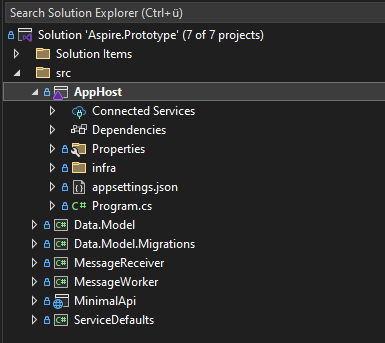
\includegraphics[scale=1]{Ressources/Bilder/Porjektstruktur.AppHost.png}\par

            Als zweites kommen die Service Defaults hinzu, welche von Aspire .Net benötigt werden. Aspire empfiehlt die Konfiguration der Service Defaults in einem eigenen Projekt zu platzieren. Wie im Bild ersichtlich wird ein Projekt \verb|ServiceDefaults| erstellt. Darin befindet sich eine Extensionmethod mit der Konfiguration der Healthcheck und Telemetrie Endpoints.

        \subsubsection{Integration des Frontends}

            Das React Frontend verwendet Facebook's Paket Manager Yarn. Aspire bietet von sich aus nur die Integration von Javascript Apps mit NPM an. Da der Source-Code von Aspire in GitHub öffentlich ist, konnte die Funktion \verb|.AddNpmApp()| analysiert werden. In diese Funktion abstrahiert das Starten einer Node App. In diesem Fall eine App basierend auf NPM. Eine React App mit Yarn ist im Kern auch eine Node App, verwendet einfach andere commands, zum installieren der Packages und Starten der App. Deshalb kann mit einer neuen Funktion das Starten einer React App mit Yarn einfach abstrahiert werden.

            \begin{minted}
            [
                breaklines,
                frame=lines,
                framesep=2mm,
                baselinestretch=1.2,
                bgcolor=bg,
                fontsize=\footnotesize,
                linenos
            ]{csharp}
public static IResourceBuilder<NodeAppResource> AddYarnApp(
    this IDistributedApplicationBuilder builder, 
    string name, 
    string workingDirectory, 
    string scriptName = "dev", 
    string[]? args = null
)
{
    string[] allArgs = args is { Length: > 0 }
        ? [scriptName, "--", .. args]
        : [scriptName];

    workingDirectory = NormalizePathForCurrentPlatform(
        Path.Combine(
            builder.AppHostDirectory, 
            workingDirectory
        )
    );
    var resource = new NodeAppResource(name, "yarn", workingDirectory);

    return builder.AddResource(resource).WithNodeDefaults().WithArgs(allArgs);
}
            \end{minted}

            Die Extension für den IDistributedApplicationBuilder \verb|.AddYarnApp()| ist von der Signatur her gleich aufgebaut wie \verb|.AddNpmApp()|. In der Methode wird auf Zeile 19 eine \verb|NodeAppRessource| instanziert. Dem Konstruktor wird der Paketmanger, respektive der Befehl für die Kommandozeile mitgegeben. Anstatt "npm" wird in dieser Methode nun "yarn" spezifiziert. 

            Im AppHost kann nun \verb|.AddYarnApp()| anstatt \verb|.AddNpmApp()| verwendet werden, um die React App mit Yarn zu starten.

            \textbf{Problemestellung Frontend Hosting}

            Im Zuge der Frontendintegration stellt sich die Frage: Wie soll das Frontend im Azure gehostet werden? Das Template ist folgendermassen konfiguriert. Lokal wird Backend und Frontend voneinander getrennt gestartet. Im Backend ist ein Proxi mit Yarp konfiguriert, welcher beim Aufruf der lokalen Backend-URI den Request an das Frontend weiterleitet. Beim Build für das Deployment wird die React App in das \verb|wwwroot| der Backend Api bereitgestellt. Das heisst, Backend und Frontend werden zusammen in einen Container oder App Service deployed. Kestrel, der ASP.NET build-in Server welcher das Backend hosted, verwendet das wwwroot als default oder fallback Route. Damit wird die React App ausgeliefert, wenn das Backend auf einer "nicht" API Route aufgerufen wird.

            Aspire verfolgt einen anderen Ansatz. Das Frontend wird sowohl lokal als auch in Azure in einen eigenen Conteiner deployed. Da auch das Template lokal das Frontend als eigenen Service integriert, funktioniert die Applikation lokal ohne weitere Anpassung. Das Deployment in Azure hingegen kann nicht einfach so erfolgen. 
            \begin{enumerate}
                \item Der Build des Frontends in das wwwroot des Backends kann nur mit einer individuell konfigurierten Pipeline realisiert werden.
                \item Die Security im Backend ist konfiguriert für ein Hosting des Frontends im Backend-Container.                
            \end{enumerate}

            Versuche die Security im Backend so anzupassen, dass Requests vom Frontend aus einem eigenen Container nicht blockiert werden, sind bisher fehlgeschlagen. Um eine Applikation nach akutellen Security Standarts aufzubauen, hat das Template sehr granulare Einstellungen. Diese Einstellungen lassen sich nicht ohne grösseren Aufwand anpassen.            

            \subsubsection{Integration des Backends und EF Migrations}

            Die Backend Api und das Projekt mit den Entity Framework Migrationen wird im AppHost referenziert. Für die Persistenz wird ausserdem eine Azure SQL Datenbank in die Komposition aufgenommen.

            \begin{minted}
            [
                breaklines,
                frame=lines,
                framesep=2mm,
                baselinestretch=1.2,
                bgcolor=bg,
                fontsize=\footnotesize,
                linenos
            ]{csharp}
var sqldb = builder.AddSqlServer("sql").AddDatabase("sqldb");

var migrations = builder.AddProject<Projects.Test_Template_React_App_Domain_Migrations>("migrations")
    .WithReference(sqldb);

var server = builder.AddProject<Projects.Test_Template_React_App_Server>("server")
    .WithReference(sqldb)
    .WithEndpoint(env: "iisSettings.iisExpress.sslPort")
    .WithExternalHttpEndpoints();
            \end{minted}

            \textbf{Azure SQL}
            
            Die SQL Datenbank wird lokal in einem Docker Container gestartet. Es ist also notwendig, dass Docker läuft damit die Aspire App ausgeführt werden kann. Aspire konfiguriert die Datenbank automatisch. Zugangsdaten und Port werden definiert und für konsumierende Services bereitgestellt.

            \textbf{Enitity Framework Migrationen}

            Im Template ist die Entity Framework Migration als .Net Projekt realisiert. Die Charakteristik des Migrationsprojekt entspricht eigentlich einem Background Serivce. Aspire empfiehlt auch die EF Migrationen in einem Background Service auszuführen. Deshalb wurde das Migrationsprojekt aus dem Template in einen Background Service umgebaut. Beim Start dieses Service, wird die Migration auf dei DB angewendet, falls noch nicht geschehen. Sollte es zu einem Fehler kommen, wird das DB Update 10 mal wiederholt. Kann die Migration nicht innerhalb von 10 Versuchen angewendet werden, wird der Background Service mit einem Fehler beendet. Ansonsten beendet der Service erfolgreich. Gerade wenn die Datenbank noch nicht vollständig gestartet wurde kann der Migration Service fehlschlagen.

            \textbf{Backend API}

            Damit das Backend sich mit der Datenbank verbindet, wird das EntityFramework Client Paket aus dem Aspire Stack verwendet
            \mint{csharp}|Aspire.Microsoft.EntityFrameworkCore.SqlServer|
            und im Startup des Backends wird die Datenbank integriert.
            
            \begin{minted}
            [
                breaklines,
                frame=lines,
                framesep=2mm,
                baselinestretch=1.2,
                bgcolor=bg,
                fontsize=\footnotesize,
                linenos
            ]{csharp}
builder.AddSqlServerDbContext<YourDbContext>("sqldb");
            \end{minted}

            Dieses Client Package sorgt für die Service Discovery des SQL Servers.

            Diese Integration hat bezüglich Datenbank Verbindung und Verwendung ohne weitere Eingriffe funktioniert. Hingegen die Verbindung zum Frontend läuft nicht reibungslos. Das Frontend kann das Backend nur via HTTP aufrufen. HTTPS funktioniert nicht, da der SSL Verbindung nicht vertraut wird. Deshalb müssen lokal HTTP Routen konfiguriert werden.

        \subsubsection{Authentifizierung}

            Microsoft Entra ID wird im Template verwendet für die Authentifizierung. Auch für die lokale Entwicklung mit dem Template, muss in Azure eine App Registration für die Applikation erstellt und im Backend konfiguriert werden. Beim Login wird das Entra ID verwendet als Identity Provider. Damit lokal, ohne Verbindung zu Azure, entickelt werden kann, müsste der Keycloak Serivce verwendet werden. Das Authentication Scheme ist auf Entra ID ausgelegt und müsste lokal umgebaut werden. Das hat aus zeitlichen Gründen nicht mehr gereicht. Die Authentifizierung konnte so lokal nicht aufgebaut werden.

        \subsubsection{Azure Key Vault}

            Das Template ist für die Verwendung von Azure Key Vault ausgelegt. Deshalb wurde der Key Vault Service von Aspire ebenfalls integriert. Leider gibt es keinen Emulator, um den Key Vault lokal zu betreiben. Es muss in Azure ein Key Vault angelegt und den Connection String im Aspire Projekt hinterlegt werden. Im Zuge der Integration von Azure Key Vault wurde festgestellt, dass es einige Azure spezifische Service gibt, welche gar nicht lokal ausgeführt werden können. Für die lokale Entwicklung müssen diese Services in Azure provisioniert und der Connection String im Projekt hinterlegt werden. Aspire verwendet dann lokal diesen manuell provisionierten Service. Wird die Aspire Applikation auf Azure ausgerollt, provisioinert Aspire den Service. So ist die lokale Umgebung tortzdem von der Azure Umgebung getrennt.

            \begin{minted}
            [
                breaklines,
                frame=lines,
                framesep=2mm,
                baselinestretch=1.2,
                bgcolor=bg,
                fontsize=\footnotesize,
                linenos
            ]{csharp}
var secrets = builder.ExecutionContext.IsPublishMode
    ? builder.AddAzureKeyVault("secrets")
    : builder.AddConnectionString("secrets");
            \end{minted}

            Wird Aspire Applikation in Azure ausgeführt ist das \verb|IsPublishMode| Property \verb|True|. In diesem Fall, wird der für die Umgebung provisionierte Key Vault verwendet. In der lokalen Umgebung wird der Connection String verwendet, um auf einen Azure Key Vault für die lokale Entwicklung zuzugreifen.

        \subsubsection{Deployment in Azure}

            Das Template verwendet für den IaC Teil Terraform. Aspire hingegen setzt auf Biceps. Biceps ist die Azure eigene IaC Sprache. Vom Template kann kein IaC Code wieder verwendet werden. Die Dokumentation von Aspire zum Thema Deployment suggeriert, dass das Deployment ohne manuellen Eingriff funktionieren sollte. Das ist nun auch die "Hoffnung", dass das Template mit der Aspire Integration einfach in Azure ausgerollt werden kann.

            Um das Deployment zu testen, in einem möglichst echten Szenario, wurde eine GitHub Action aufgebaut. Dazu gibt es von Aspire Beispiele. Mit wenigen Anpassungen konnte das Beispiel übernommen werden. Die Azure Developer CLI bietet die Möglichkeit das Deployment via GitHub Action einzurichten. Das Empfiehlt sich auch, da in Azure der nötige Service Principal angelegt wird und in GitHub die Ids und Secrets angelegt. Ohne diese Konfiguration kann die GitHub Action nicht auf die Azure Ressource zugreifen und Infrastruktur provisionieren. Danach funktioniert das Deployment auch und in Azure wird die ganze Infrastruktur provisioniert und der App Code deployed.

        \subsubsection{Ergebnis der Integration}
            Leider konnte die Aspire und das Kickstarter Template nicht in der Zeit miteinander Integriert werden. Das Kickstarter Template ist schon so ausgeklügelt, dass es einen grossen Aufwand bedeuten würde, alle Aspekte für Aspire anzupassen. Dies wäre aber nötig, damit das Aspire Template funktionieren würde. Ausserdem sind einige Azure Services gar nicht lokal verfügbar. Das wäre aber ein wichtiger Aspekt gewesen, dass Azur Lösungen, offline und lokal entwickelt werden können. Das ist im aktuellen Stand von Aspire nicht gegeben. 

            Dazu kommt das Deployment ist im Template bis ins kleinste Detail mit IaC abgebildet. Da Aspire auf eine andere IaC Sprache setzt, kann der IaC Code vom Template nicht übernommen werden. Um den Detailgrad des Templates nun mit Aspire zu erreichen, müsste so tief in den von Aspire generierten Code eingreifen, dass der Vorteil von Aspire nicht mehr gegeben ist. Es war nicht möglich den Konfigurationsgrad des Templates mit Aspire zu erreichen. Dazu müsste mehr Aufwand in den IaC code gesteckt werden.
            
    \subsection{Iteration 2: Erkenntnisse}

        \subsubsection{Aspire Tutorials}
            Die Aspire Dokumentation enthält sehr viele Tutorials und Beispiele. Zu jedem Service gibt es Beispiele, wie der Service integriert wird. Das ist für den Aufbau von Know-How sehr hilfreich. Allerdings zeigen die Beispiele oft nur eine einfache, für den Service zugeschnittene Situation. Je mehr Services und Anforderungen zu einer Lösung dazu kommen, um so komplexer wird die Komposition und Konfiguration. Hier helfen dann auch Tutorials nicht mehr weiter und die Knowledgebase im Internet ist noch nicht so gross, so dass noch viel Try and Error nötig ist.

        \subsubsection{Lokale Entwicklung}
            Lokal kann das Template mit Aspire in gewissen Aspekten ergänzt und ausgeführt werden. Da die Authentifizierung nicht zu 100\% zum Laufen gebracht wurde, waren gewisse Teile der Applikation nicht zugänglich. Da der Azure Key Vault und auch Azure AppInsights für das Logging gar nicht lokal ausgeführt werden, sondern in Azure provisioniert werden müssen, ist eine offline Entwicklung gar nicht möglich. Da Aspire das Startprojekt ist und das Ausführen der Serivces übernimmt, vereinfacht Aspire die lokale Entwicklung. Entweder startet der Entwickler alle Services manuell oder schreibt ein Skript, welches die Services startet. Aspire übernimmt diesen Part und erleichtert so das lokale Entwickeln.

        \subsubsection{Deployment auf Azure}
            Die wichtigste Erkenntnis beim Deployment auf Azure ist, Aspire übernimmt fast alles. Falls das ausreicht ist das Deployment einfach. Werden Services ergänzt oder verändert, erkennt Aspire selber ob ein Service neu provisioniert werden muss oder ob nur ein Deployment des Codes nötig ist. Sobald man aber manuell in das Deployment eingreift muss man extrem aufpassen, dass Aspire in der Lage bleibt, Änderungen den richtigen Services zuzuordnen. Sonst versucht Aspire einfach einen neuen Service hochzufahren. Das kann dazu führen das verwaiste Services übrig bleiben oder das Provisioning fehlschlägt, weil zum Beispiel Aspire versucht einen Service mit einem Namen zu provisionieren, welcher schon existiert. Das führt zu einem Fehlschlag des Deployments.

    \subsection{Iteration 3: Aufbau eines neuen Protoypes}
        Damit im Rahmen der Arbeit trotzdem ein vorzeigbares Ergebnis vorliegt und Aspire .Net vorgeführt werden kann, wird ein Prototyp mit einem kleinen Use-Case aufgebaut.
        
        \subsubsection{Anforderungen an den Prototyp}
            Im Prototyp soll die Funktionsweise von Aspire vorgestellt werden. Es soll eine Komposition gezeigt werden mit verschieden Services, Backend, Frontend ein oder zwei Azure Services. Damit soll die lokale Entwicklung und ein Deployment in Azure demonstriert werden.

        \subsubsection{Architektur des Prototyps}
            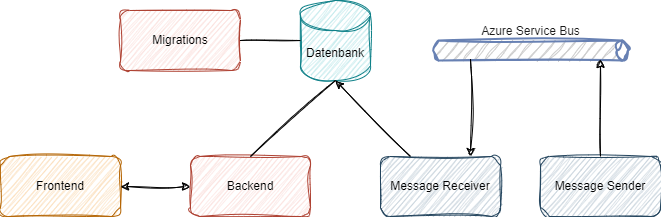
\includegraphics[scale=0.55]{Ressources/Bilder/Architektur.Prototyp.drawio.png}

            \textbf{Frontend}

            Das Frontend ist ein einfaches Angular Frontend, welches eine Tabelle mit Daten aus dem Backend darstellt.

            \textbf{Backend}

            Das Backend ist eine .Net Minimal Api und bietet einen Endpoint für das Frontend, um die Daten aus der Datenbank für das Frontend bereit zu stellen. 

            \textbf{Datenbank}

            Die Datenbank ist ein PostgreSQL und wird mit Entity Framework Core für PostgreSQL im Backend und im Message Receiver angebunden.

            \textbf{Migrations}

            Dies ist ein Background Service mit den Entity Framework Migrationen. Dieser Service versucht die Migration auf die Datenbank anzuwenden, wenn er gestartet wird.

            \textbf{Message Sender}
            
            Der Message Sender ist ein Background Service welcher in einem eingestellten Zeitinterval eine Message an den Azure Serivce Bus sendet.

            \textbf{Azure Service Bus}
            
            Der Azure Service Bus ist ein klassischer Service für das Message queuing.

            \textbf{Message Receiver}

            Der Message Receiver ist auch ein Background Service, welcher die Messages aus dem Azure Serice Bus entgegen nimmt und in die Datenbank speichert.

        \subsubsection{Aufbau des Prototypen}

            In diesem Abschnitt sind die interessantesten Aspekte des Prototyps beschrieben. Der gesamte Code ist in GitHub und kann dort besichtigt werden.
            \mint{csharp}|https://github.com/zuercheram/aspire-prototype/tree/master|

            \begin{minted}
            [
                breaklines,
                frame=lines,
                framesep=2mm,
                baselinestretch=1.2,
                bgcolor=bg,
                fontsize=\footnotesize,
                linenos
            ]{csharp}
var builder = DistributedApplication.CreateBuilder(args);

var postgres = builder.AddPostgres("postgres").PublishAsAzurePostgresFlexibleServer();
var postgresdb = postgres.AddDatabase("postgresdb");

var serviceBus = builder.ExecutionContext.IsPublishMode
    ? builder.AddAzureServiceBus("messaging")
    : builder.AddConnectionString("messaging");

builder.AddProject<MessageWorker>("messageworker")
    .WithReference(serviceBus);

var weatherApi = builder.AddProject<MinimalApi>("messagesapi")
    .WithReference(postgresdb)
    .WithExternalHttpEndpoints();

builder.AddNpmApp("angular", "../Frontend")
    .WithReference(weatherApi)
    .WithHttpEndpoint(env: "PORT")
    .WithExternalHttpEndpoints()
    .PublishAsDockerFile();

builder.AddProject<MessageReceiver>("messagereceiver")
    .WithReference(postgresdb)
    .WithReference(serviceBus);

builder.AddProject<Data_Model_Migrations>("data-model-migrations")
    .WithReference(postgresdb);

builder.Build().Run();
            \end{minted}

            Der Code Abschnitt ist die gesamte Komposition für die Aspire App. Alle indiviudellen Services, das Frontend, Azure Service Bus und die EF Migration wird in diesem Code definiert. Mit \verb|.WithReference()| werden die Services miteinander "Verknüpft". Dies ist für die Service Discovery von Aspire wichtig.

            

    \subsection{Iteration 3: Erkenntnisse}



